\documentclass[11pt]{report}

\usepackage[left=2cm, right=2cm, top=2cm]{geometry}
\usepackage[spanish]{babel}
\usepackage[utf8]{inputenc}
\usepackage{amsmath}
\usepackage{amssymb}
\usepackage{graphicx}
\graphicspath{ {images/} }

\begin{document}

%Macros generales
\newcommand{\BP}[1]{\bigg( #1 \bigg)} %Paréntesis demasiado grandes
\newcommand{\Bp}[1]{\Big( #1 \Big)} %Paréntesis muy grandes
\newcommand{\bp}[1]{\big( #1 \big)} %Paréntesis grandes pero no tanto
\newcommand*\Eval[3]{\left.#1\right\rvert_{#2}^{#3}} %Evaluación

%Macros específicos
\newcommand{\tsint}[1]{\int_0^{#1}} %Integral para el ejercicio 37, lím. inf. 0.

\begin{center}
		\textsc{\huge Matemáticas para las \\Ciencias Aplicadas III \\ Tarea 2\\}
		\textbf{Alan Arteaga, Alma Sánchez, Jerónimo Almeida}
\end{center}

\textbf{El cuaderno dónde se resuelven los problemas evaluados en un CAS se encuentran
		en la siguiente liga:\\
		$https://github.com/chiknahuikoatl/Tarea\_MCA\_III\\
		/blob/master/Tarea\_MCA\_III/Tarea\_2/Tarea\_2.nb$}

\textbf{Anton-Bivens-Davis} \\

\textbf{Sección 14.2} \\
\textbf{15-18} Evaluate the double integral in two ways using iterated integrals:
(a) viewing $R$ as a type I region, and (b) viewing $R$ as a type II region.

\textbf{18.} \\

$ {\displaystyle \iint \limits_R } \, y \, \, \text dA; \, R$ is the region in the first
quadrant enclosed between the circle $x^2 + y^2 = 25$ and the line $x + y = 5$. \\
Entonces la integral al definir los límites de integración, tenemos:
$${\displaystyle \iint \limits_R } \, y \, \, \ text dA = \, \int_{0}^{5} \int_{5-x}^{\sqrt{25 - x^2}} \, y\,dy\,dx$$

Integramos con respecto a $y$
$$ = \int_{0}^{5} \left[ \frac{y^2}{2} \right]_{5-x}^{\sqrt{25 - x^2}} \, dx$$

Sacamos el $\frac{1}{2}$, evaluamos y resolvemos las operaciones
$$ = \frac{1}{2} \int_{0}^{5} \left(25-x^2\right) - \left(5-x\right)^2 \, dx$$

Llegamos a
$$ = \frac{1}{2} \int_{0}^{5} 10x - 2x^2 \, dx$$


Calculando las integrales por separado
$$ = \frac{1}{2} \int 10x\, dx - \int 2x^2\,dx$$
$$ = 10 \int x\,dx = 10 * \frac{x^{1+1}}{1+1} = 5x^2$$
$$ = 2 \int x^2 \, dx = 2 * \frac{x^2+1}{2+1} = \frac{2x^3}{3}$$
$$ =  5x^2 - \frac{2x^2}{3}$$

Entonces tenemos que calcular los límites tal que
$$\int_{0}^{5} 10-2x^2\,dx = \frac{125}{3}$$

Por lo tanto
$$\frac{1}{2} * \frac{125}{3} = \frac{125}{6}$$


Ahora la otra región

$${\displaystyle \iint \limits_R } \, y \, \, \ text dA = \, \int_{0}^{5} \int_{5-x}^{\sqrt{25 - x^2}} \, y\,dy\,dx$$
$$ = \int_{0}^{5} y [\sqrt{25-y^2} - (5-y)] \, dy$$

Que lo podemos separar
$$ = \int_{0}^{5} y \sqrt{25-y^2} dy - \int_{0}^{5} y(5-y) \, dy $$
$$ = \frac{125}{3}$$

Por lo tanto
$$\frac{125}{3} - \frac{125}{6} = \frac{125}{6}$$



\textbf{19-24.} Evaluate the double integral. \\

\textbf{22.} $ {\displaystyle \iint \limits_R } \, x \, \, \text dA; \, R$ is the region
enclosed by $y = sin^{-1} x, x = \frac{1}{\sqrt{2}},$ and $y = 0$. \\

Notamos que la región R es el área entre las curvas:

\begin{figure}[h]
%\includegraphics[scale=0.5]{images/img3.png}
\centering
\end{figure}

Entonces, la integral iterada es:

\[ \int \limits_0^{\frac{1}{\sqrt{2}}} \int \limits_0^{\arcsin{x}} x \, \text dy \text dx \]

Resolviendo la integral interna:

\begin{equation}
\begin{split}
        \int \limits_0^{\arcsin{x}} x \, \text dy & =  x \int \limits_0^{\arcsin{x}} \, \text dy \\ \notag
        & = x (\arcsin{x})
\end{split}
\end{equation}

Entonces:

\begin{equation}
\begin{split}
        \int \limits_0^{\frac{1}{\sqrt{2}}}
        \int \limits_0^{\arcsin{x}} x \, \text dy \text dx &=
        \int \limits_0^{\frac{1}{\sqrt{2}}} x (\arcsin{x}) \, \text dx \\ \notag
\end{split}
\end{equation}

Integrando por partes:

\begin{equation}
\begin{split}
        u = \arcsin{x} \rightarrow du = \frac{1}{\sqrt{1 - x^2}} dx \\ \notag
        dv = x dx \rightarrow v = \frac{x^2}{2}
\end{split}
\end{equation}

Entonces:

\begin{equation}
\begin{split}
        \int \limits_0^{\frac{1}{\sqrt{2}}} x (\arcsin{x}) \, \text dx
        &= \arcsin{(x)} \frac{x^2}{2} \Bigg|_0^{\frac{1}{\sqrt{2}}}
        - \int \limits_0^{\frac{1}{\sqrt{2}}} \frac{x^2}{2} \frac{1}{\sqrt{1 - x^2}} dx \\ \notag
\end{split}
\end{equation}

Donde:

\begin{equation}
\begin{split}
        \int \limits_0^{\frac{1}{\sqrt{2}}} \frac{x^2}{2} \frac{1}{\sqrt{1 - x^2}} dx
        &= \frac{1}{2} \int \limits_0^{\frac{1}{\sqrt{2}}} \frac{x^2}{\sqrt{1 - x^2}} dx \notag
\end{split}
\end{equation}

Por sustitución trigonométrica:

\begin{equation}
\begin{split}
        x = \sin{(\theta)} \rightarrow \frac{dx}{d\theta} = \cos{(\theta)}
        \rightarrow dx = \cos{(\theta)} d\theta \\ \notag
\end{split}
\end{equation}
\begin{equation}
\begin{split}
        \cos{(\theta)} = \sqrt{1 - x^2} \\ \notag
        \sin{(\theta)} = x \rightarrow \sin^2{(\theta)} = x^2
\end{split}
\end{equation}
\begin{equation}
\begin{split}
        x = \sin{(\theta)} \rightarrow \frac{1}{\sqrt{2}} = \frac{\sqrt{2}}{2} = \sin{(\theta)}
        \rightarrow \theta_1 = \frac{\pi}{4} \\ \notag
        x = \sin{(\theta)} \rightarrow 0 = \sin{(\theta)}
        \rightarrow \theta_2 = 0 \notag
\end{split}
\end{equation}

Entonces:

\begin{equation}
\begin{split}
        \frac{1}{2} \int \limits_0^{\frac{\pi}{4}} \frac{x^2}{\sqrt{1 - x^2}} dx \notag
        &= \frac{1}{2} \int \limits_0^{\frac{\pi}{4}} \frac{\sin^2{\theta}}{\cos{\theta}} \cos{\theta} d\theta \\ \notag
        &= \frac{1}{2} \int \limits_0^{\frac{\pi}{4}} \sin^2{\theta} d\theta \\ \notag
        &= \frac{1}{2} \int \limits_0^{\frac{\pi}{4}} \frac{1 - \cos{2\theta}}{2} d\theta \\ \notag
        &= \frac{1}{4} \int \limits_0^{\frac{\pi}{4}} 1 - \cos{2\theta} d\theta \\ \notag
        &= \frac{1}{4} \left( \theta - \frac{1}{2} \sin{2\theta} \right) \Bigg|_0^{\frac{\pi}{4}}
\end{split}
\end{equation}
\begin{equation}
\begin{split}
        &= \frac{1}{4} \left( \frac{\pi}{4} - \frac{1}{2}\sin{\left(\frac{2\pi}{4} \right)} - 0 + \frac{1}{2} \sin{(2 \cdot 0)} \right)  \\ \notag
        &= \frac{1}{4} \left( \frac{\pi}{4} - \frac{1}{2}\sin{\left(\frac{\pi}{2} \right)} + \frac{1}{2} \sin{0} \right)  \\ \notag
        &= \frac{1}{4} \left( \frac{\pi}{4} - \frac{1}{2} \right)  \\ \notag
        &= \frac{\pi}{16} - \frac{1}{8}  \\ \notag
        &= \frac{\pi - 2}{16}
\end{split}
\end{equation}

Entonces:

\begin{equation}
\begin{split}
        \int \limits_0^{\frac{1}{\sqrt{2}}} x (\arcsin{x}) \, \text dx
        &= \arcsin{(x)} \frac{x^2}{2} \Bigg|_0^{\frac{1}{\sqrt{2}}}
        - \int \limits_0^{\frac{1}{\sqrt{2}}} \frac{x^2}{2} \frac{1}{\sqrt{1 - x^2}} dx \\ \notag
        &= \arcsin{(x)} \frac{x^2}{2} \Bigg|_0^{\frac{1}{\sqrt{2}}} - \frac{\pi - 2}{16} \\ \notag
        &= \arcsin{ \left( \frac{1}{\sqrt{2}} \right)} \frac{ \left( \frac{1}{\sqrt{2}} \right)^2}{2}
        - \arcsin{(0)} \frac{(0)^2}{2} - \frac{\pi - 2}{16} \\ \notag
        &=  \frac{1}{4} \arcsin{ \left( \frac{1}{\sqrt{2}} \right)}
         - \frac{\pi - 2}{16} \\ \notag
        &=  \frac{1}{4} \left( \arcsin{ \left( \frac{1}{\sqrt{2}} \right)}
         - \frac{\pi - 2}{4} \right) = 0.125 u^2 \\ \notag
\end{split}
\end{equation}


\textbf{28.} \\
\begin{itemize}
	\item[(a)] {
		By hand or with the help of a graphing utility, make a sketch of the region
		$R$ enclosed between the curves $y = 4x^3 - x^4$ and $y = 3 - 4x + 4x^2$. \\
		\begin{figure}
			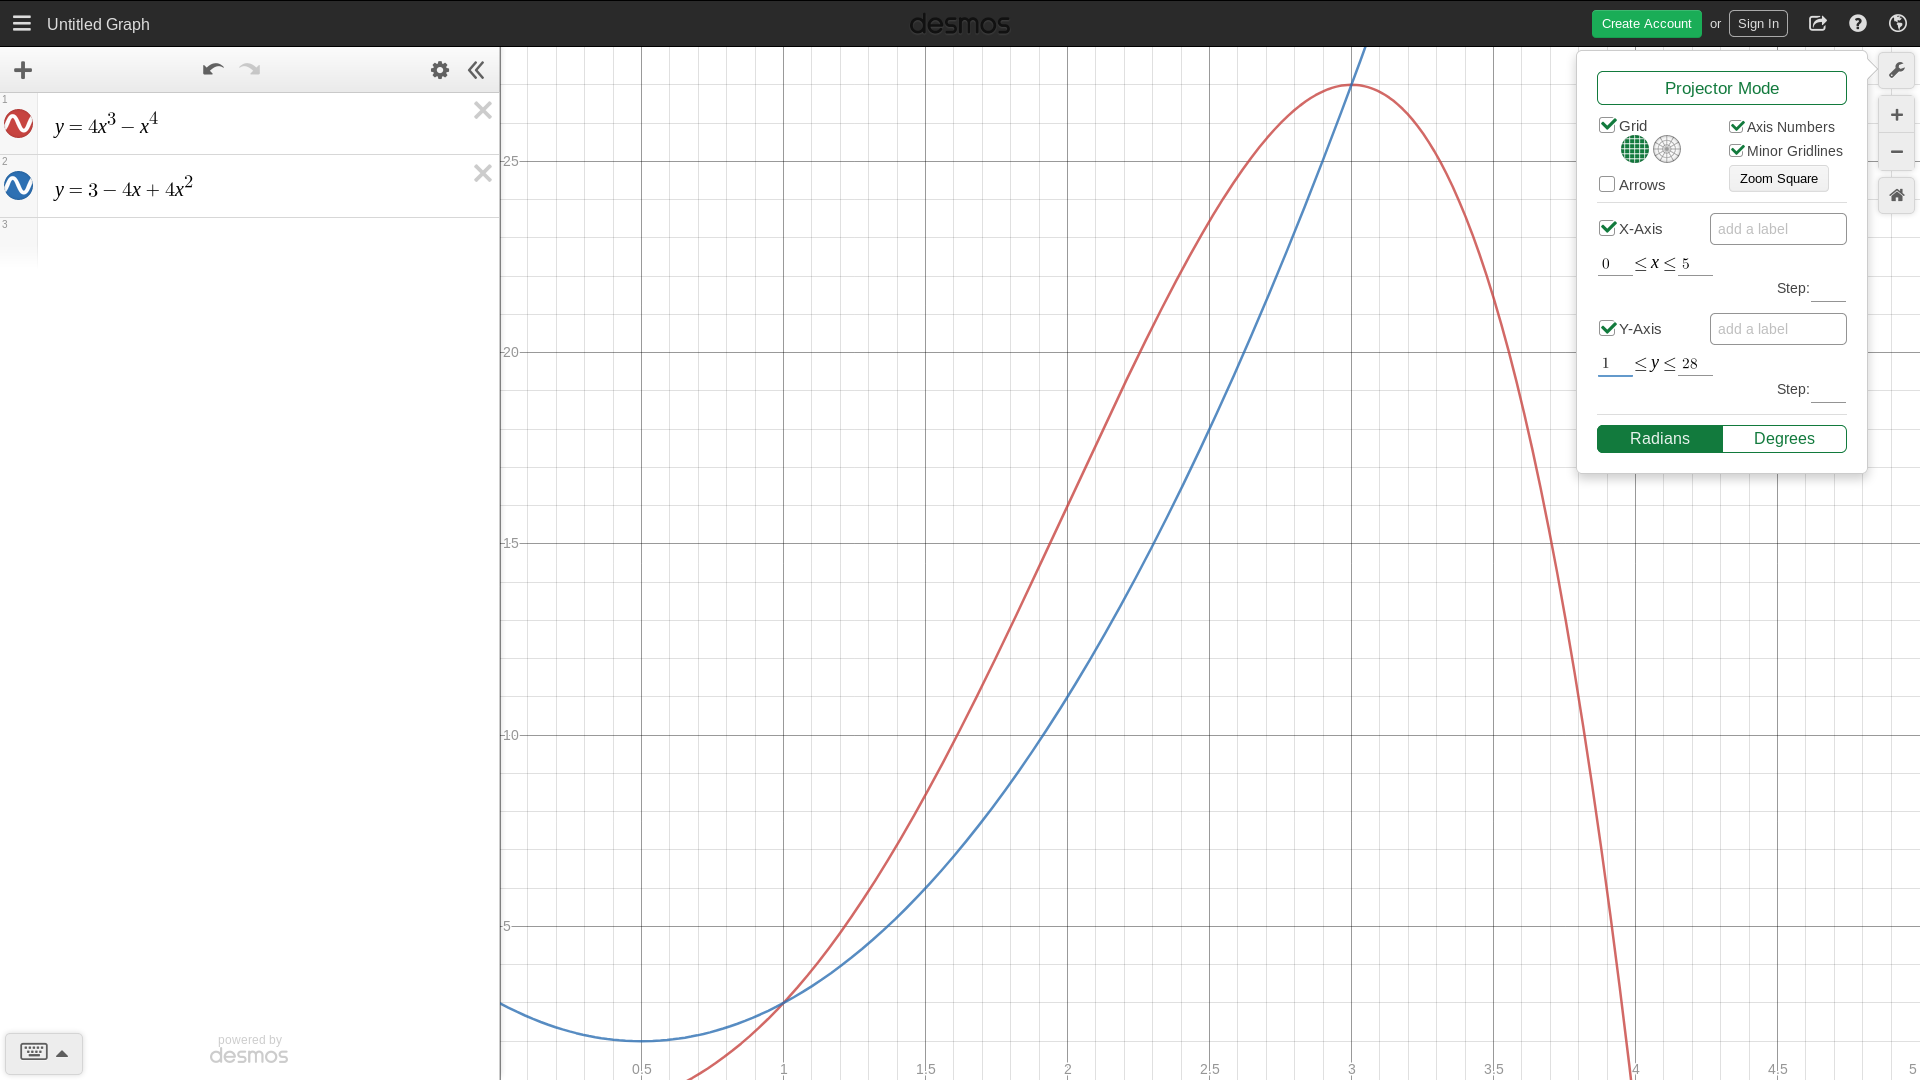
\includegraphics[scale=0.2]{A-B-D_14_2_28_a.png}
			\caption{Gráfica de las funciones dadas para el ejercicio 14.2.28.}
			\centering
		\end{figure}
		\begin{figure}
			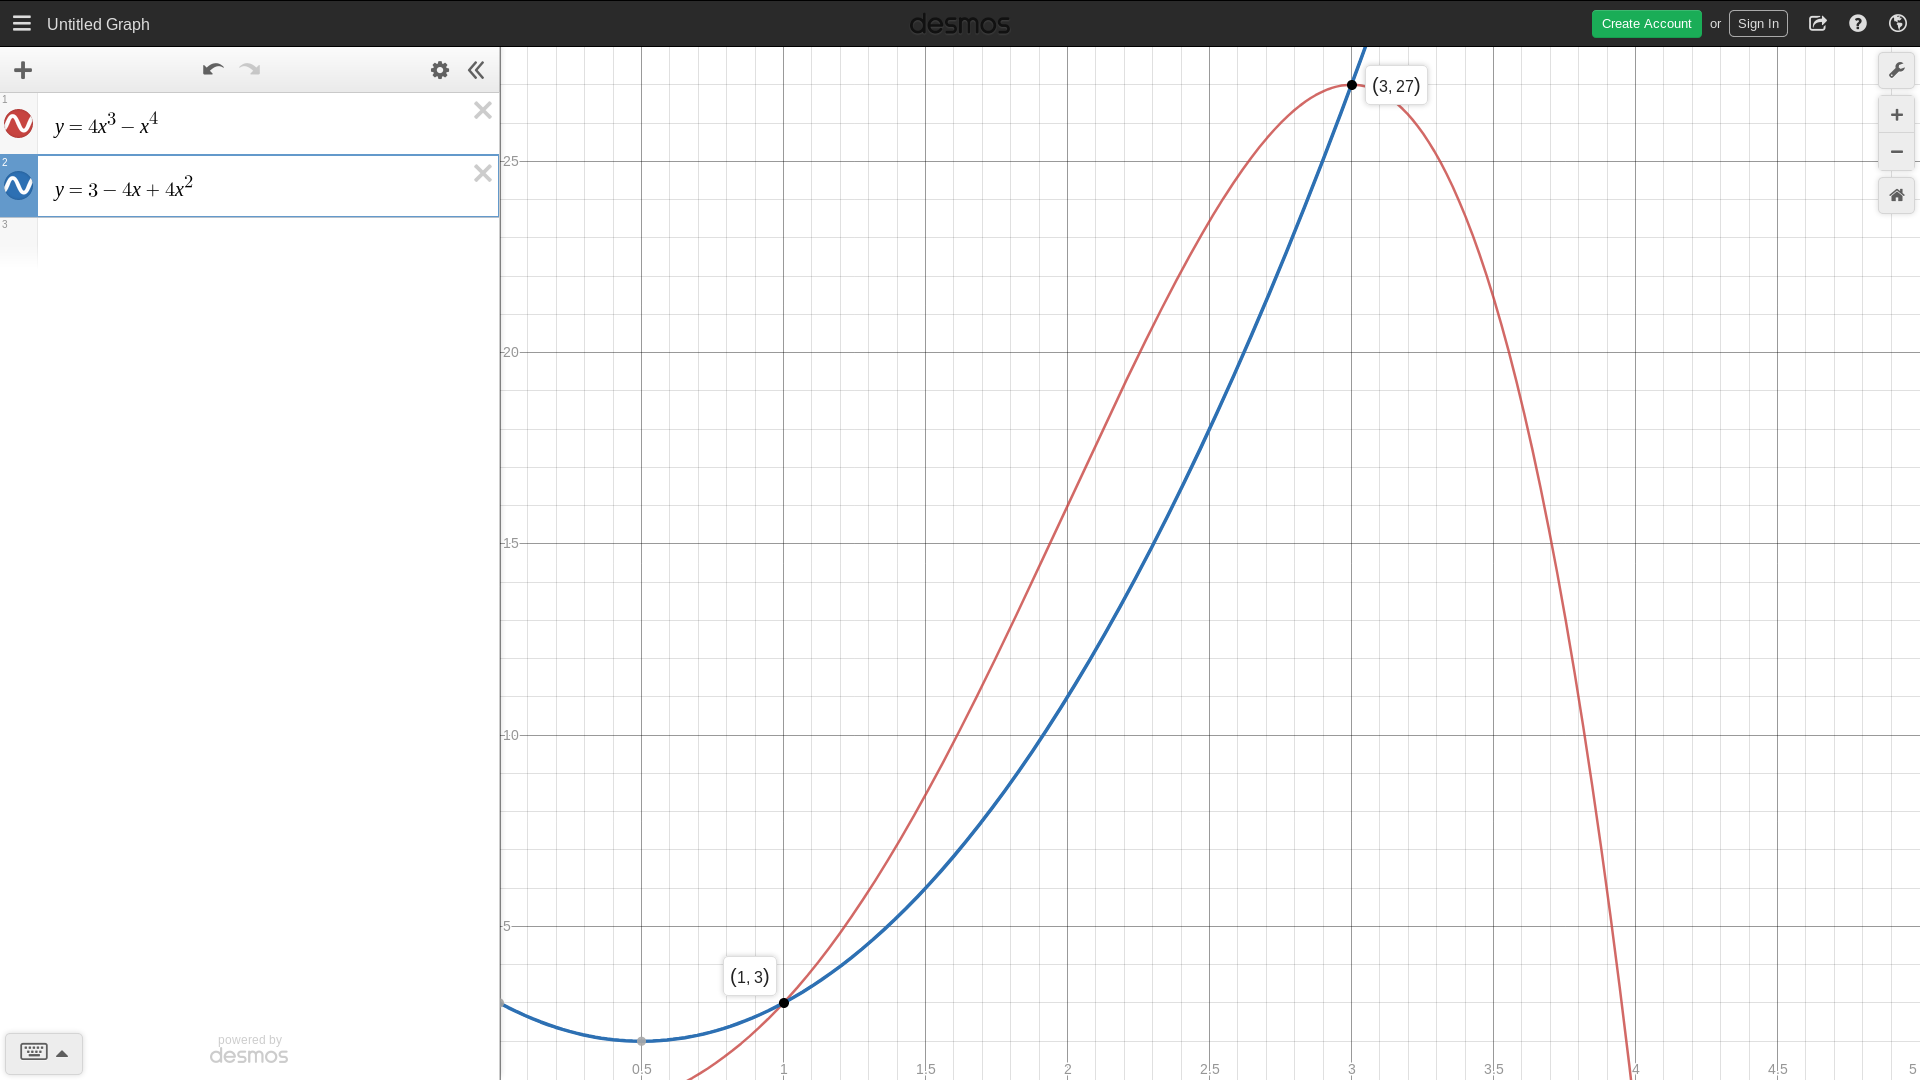
\includegraphics[scale=0.2]{images/A-B-D_14_2_28_b.png}
			\caption{Gráfica de las funciones dadas para el ejercicio 14.2.28 con los puntos
					dónde se intersectan las gráficas.}
			\centering
		\end{figure}
	}

	\item[(b)]{
		Find the intersection of the curves in part (a)\\
		Según las gráficas del inciso anterior pdemos ver que las curvas se intersectan
		en los puntos $$x=1,\ 3\ \ \&\ \ y=3,\ 27$$
	}
	\item[(c)]{
		Find $ {\displaystyle \iint \limits_R } \, x \, \, \text dA $ \\
		\begin{equation}
		\begin{split}
			\int\int_Rx &=\int_1^3\int_{3-4x+4x^2}^{4x^3-x^4}xdydx\\
				   	   &=\int_1^3yx\Big|_{3-4x+4x^2}^{4x^3-x^4}dx\\
					    &=\int_1^3 (4x^4-x^5-3x+4x^2-4x^3)dx\\
						&=(\tfrac{4x^5}{5}-\tfrac{x^6}{6}-\tfrac{3x^2}{2}+\tfrac{4x^3}{3}-x^4)\Big|_1^3\\
						&=\tfrac{972}{5}-\tfrac{243}{2}-\tfrac{27}{2}+36-81-\tfrac{4}{5}+\tfrac{1}{6}+\tfrac{3}{2}-\tfrac{4}{3}+1\\
						&=\tfrac{968}{5}-135+36-81+\tfrac{1}{6}+\tfrac{3}{2}-\tfrac{4}{3}+1\\
						&=\tfrac{968}{5}-179+\tfrac{1}{6}+\tfrac{3}{2}-\tfrac{4}{3}\\
						&=\tfrac{968}{5}-179+\tfrac{1+9-8}{6}\\
						&=\tfrac{968}{5}-179+\tfrac{1}{3}\\
						&=\tfrac{2904}{15}-\tfrac{2685}{15}+\tfrac{5}{15}\\
						&=\tfrac{2904-2685+5}{15}\\
						&=\tfrac{224}{15}\\
			\end{split}
		\end{equation}
	}

\end{itemize}

\textbf{37-38} Use double integration to find the volume of the solid. \\

\textbf{37.} \\

\begin{figure}[h]
%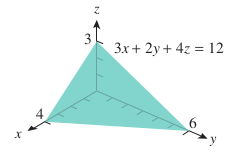
\includegraphics[scale=0.5]{images/img1.png}
\centering
\end{figure}

Tenemos que integrar
\[\int_0^4 \int_0^{6-3x/2}\left( 3- \frac{3x}{4}- \frac{y}{2} \right) dy dx\]
Comenzamos a integrar respecto a $y$, por lo que pasa como constantes $(3- \frac{3x}{4})$ multiplicado por $y$, entonces :
\[\int_0^4 y \left( 3- \frac{3x}{4}\right)- \frac{y^2}{4} \vert_0^{6-3x/2} dx\]
Evaluamos:
\[\int_0^4 \left(6 - \frac{3x}{2} \right)\left( 3- \frac{3x}{4}\right)- \frac{\left(6 - \frac{3x}{2} \right)^2}{4} dx = 12\]

\textbf{57.} Try to evaluate the integral with a CAS using the stated order of
integration, and then by reversing the order of integration.\\

(a) \[\displaystyle \int \limits_0^4 \int \limits_{\sqrt{x}}^2 \, \sin{\pi y^3} \, \,  \]

(b) \[\displaystyle \int \limits_0^1 \int \limits_{sin^{-1}y}^{\frac{\pi}{2}}  \, \sec{\cos{x}}^2 \, \, \text{dx} \text{dy} \]

\textbf{59.} Evaluate $ {\displaystyle \iint \limits_R } \, xy^2 \, \, \text dA $ over
the region R shown in the accompanying figure. \\
\begin{figure}[h]
%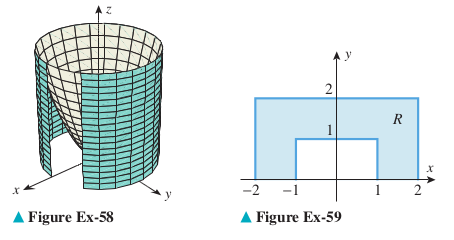
\includegraphics[scale=0.5]{images/img2.png}
\centering
\end{figure}

Se tiene que la evaluación de la integral doble para la región (separando la
región a integrar en tres segmentos)está dada por:
	$$ \int_{-2}^{-1}\int_{0}^{2} xy^2 dydx +
	   \int_{-1}^{1}\int_{1}^{2} xy^2 dydx +
	   \int_{1}^{2}\int_{0}^{2} xy^2 dydx $$

luego, esto es equivalente a :
	$$ \int_{-2}^{-1} x \int_{0}^{2} y^2 dydx +
		\int_{-1}^{1} x \int_{1}^{2} y^2 dydx +
		\int_{1}^{2} x \int_{0}^{2} y^2 dydx $$

	$$ \int_{-2}^{-1} x \Eval{\frac{y^3}{3}}{0}{2} dx +
		\int_{-1}^{1} x \Eval{\frac{y^3}{3}}{1}{2} dx +
		\int_{1}^{2} x \Eval{\frac{y^3}{3}}{0}{2} dx $$

	$$ \int_{-2}^{-1} x \frac{8}{3} dx +
		\int_{-1}^{1} x \frac{7}{3} dx +
		\int_{1}^{2} x \frac{8}{3} dx $$

	$$  \frac{8}{3} \int_{-2}^{-1} x dx +
		\frac{7}{3} \int_{-1}^{1} x  dx +
		\frac{8}{3} \int_{1}^{2} x  dx $$

	$$  \frac{8}{3} \Eval{\frac{x^2}{2}}{-2}{-1} +
		\frac{7}{3} \Eval{\frac{x^2}{2}}{-1}{1} +
		\frac{8}{3} \Eval{\frac{x^2}{2}}{1}{2} $$

	$$  \frac{8}{3} \Bp{- \frac{3}{2}} +
		\frac{7}{3} \Bp{\frac{0}{2}} +
		\frac{8}{3} \Bp{\frac{3}{2}} =
		\frac{8}{3} \Bp{\frac{3}{2}} - \frac{8}{3} \Bp{\frac{3}{2}} = 0 $$

así, se sigue que la evaluación de la integral en la región dada es igual a $0$.\\

\textbf{63.} Suppose that the temperature in degrees Celsius at a point $(x, y)$
on a flat metal plate is $T(x, y) = 5xy + x^2 $, where $x$ and $y$ are in meters.
Find the average temperature of the diamond-shaped portion of the plate for which
$|2x + y| \leq 4$ and $|2x - y| \leq 4$. \\

\textbf{Sección 14.5} \\

\textbf{12.} $ {\displaystyle \iiint \limits_G } \, \cos{\frac{z}{y}} \, \, \text dV $,
where $G$ is the solid defined by the inequalities
$\frac{\pi}{6} \leq y \leq \frac{\pi}{2}, y \leq x \leq \frac{\pi}{2}, 0 \leq z \leq xy$. \\

Entonces, la integral iterada es:

\begin{equation}
\begin{split}
        \int \limits_{\frac{\pi}{6}}^{\frac{\pi}{2}}
        \int \limits_{y}^{\frac{\pi}{2}}
        \int \limits_0^{xy} \cos{\frac{z}{y}} \, \text dz \, \text dx \, \text dy
        &=
        \int \limits_{\frac{\pi}{6}}^{\frac{\pi}{2}}
        \int \limits_{y}^{\frac{\pi}{2}}
        y \sin{\frac{z}{y}} \Bigg|_0^{xy}  \, \text dx \, \text dy \\ \notag
        &=
        \int \limits_{\frac{\pi}{6}}^{\frac{\pi}{2}}
        \int \limits_{y}^{\frac{\pi}{2}}
        y \left( \sin{\frac{xy}{y}} - \sin{\frac{0}{y}} \right) \, \text dx \, \text dy \\ \notag
        &=
        \int \limits_{\frac{\pi}{6}}^{\frac{\pi}{2}}
        \int \limits_{y}^{\frac{\pi}{2}}
        y \sin{x} \, \text dx \, \text dy
        =
        \int \limits_{\frac{\pi}{6}}^{\frac{\pi}{2}} y
        \int \limits_{y}^{\frac{\pi}{2}}
        \sin{x} \, \text dx \, \text dy \\ \notag
        &=
        \int \limits_{\frac{\pi}{6}}^{\frac{\pi}{2}} y
        \left(-\cos{x} \Bigg|_y^{\frac{\pi}{2}} \right) \, \text dy \\ \notag
        &=
        \int \limits_{\frac{\pi}{6}}^{\frac{\pi}{2}} y
        \left(-\cos{\frac{\pi}{2}} + \cos{y} \right) \, \text dy \\ \notag
        &=
        \int \limits_{\frac{\pi}{6}}^{\frac{\pi}{2}} y
        \cos{y} \, \text dy \\ \notag
\end{split}
\end{equation}

Integrando por partes:

\begin{equation}
\begin{split}
        u = y \rightarrow du = dy \\ \notag
        dv = \cos{y} dy \rightarrow v = \sin{y}
\end{split}
\end{equation}

Entonces:

\begin{equation}
\begin{split}
        \int \limits_{\frac{\pi}{6}}^{\frac{\pi}{2}} y
        \cos{y} \, \text dy
        &= y \sin{y} \Big|_{\frac{\pi}{6}}^{\frac{\pi}{2}}
        - \int \limits_{\frac{\pi}{6}}^{\frac{\pi}{2}} \sin{y} dy \\ \notag
        &= y \sin{y} \Big|_{\frac{\pi}{6}}^{\frac{\pi}{2}} - \left( - \cos{y} \Big|_{\frac{\pi}{6}}^{\frac{\pi}{2}} \right) \\ \notag
        &= y \sin{y} \Big|_{\frac{\pi}{6}}^{\frac{\pi}{2}} - \left( - \cos{(\frac{\pi}{2})} + \cos{(\frac{\pi}{6})} \right) \\ \notag
        &= \frac{\pi}{2} \sin{\left( \frac{\pi}{2} \right)} - \frac{\pi}{6} \sin{\left( \frac{\pi}{6} \right)}
        - \cos{\left( \frac{\pi}{6} \right)} \\ \notag
        &= \frac{\pi}{2} - \frac{\pi}{6} \sin{\left( \frac{\pi}{6} \right)}
        - \cos{\left( \frac{\pi}{6} \right)} \approx 0.443 u^3 \\ \notag
\end{split}
\end{equation}

\textbf{37.} Let $G$ be the tetrahedron in the first octant bounded by the
coordinate planes and the plane \\

\[ \tfrac{x}{a} + \tfrac{y}{b} + \tfrac{z}{c} = 1, (a > 0, b > 0, c > 0) \]

(a) List six different iterated integrals that represent the volume of $G$. \\
\begin{itemize}
	\item[i] \[V_G(xyz)=\tsint{a}\tsint{(b(1-\tfrac{x}{a}))}\tsint{(c(1-\tfrac{x}{a}-\tfrac{y}{b}))}dzdydx\]
	\item[ii] \[V_G(xzy)=\tsint{a}\tsint{(c(1-\tfrac{x}{a}))}\tsint{(b(1-\tfrac{x}{a}-\tfrac{z}{c}))}dydzdx\]
	\item[iii] \[V_G(yxz)=\tsint{b}\tsint{(a(1-\tfrac{y}{b}))}\tsint{(c(1-\tfrac{x}{a}-\tfrac{y}{b}))}dzdxdy\]
	\item[iv] \[V_G(yzx)=\tsint{b}\tsint{(c(1-\tfrac{y}{b}))}\tsint{(a(1-\tfrac{z}{c}-\tfrac{y}{b}))}dxdzdy\]
	\item[v] \[V_G(zxy)=\tsint{c}\tsint{(a(1-\tfrac{z}{c}))}\tsint{(b(1-\tfrac{x}{a}-\tfrac{y}{b}))}dydxdz\]
	\item[vi] \[V_G(zyx)=\tsint{c}\tsint{(b(1-\tfrac{z}{c}))}\tsint{(a(1-\tfrac{z}{c}-\tfrac{y}{b}))}dxdydz\]
\end{itemize}

(b) Evaluate any one of the six to show that the volume of $G$ is $\tfrac{1}{6} abc$. \\
\begin{equation}
	\begin{split}
		V_G(xyz)&=\tsint{c}\tsint{b(1-\tfrac{z}{c})}\tsint{a(1-\tfrac{z}{c}-\tfrac{y}{b})}dxdydz\\
				&=\tsint{c}\tsint{b(1-\tfrac{z}{c})}x\Big|_0^{a(1-\tfrac{z}{c}-\tfrac{y}{b})}dydz\\
				&=\tsint{c}\tsint{b(1-\tfrac{z}{c})}a(1-\tfrac{z}{c}-\tfrac{y}{b})dydz\\
				&=a\tsint{c}\tsint{b(1-\tfrac{z}{c})}(1-\tfrac{z}{c}-\tfrac{y}{b})dydz\\
				&=a\tsint{c}(y-\tfrac{yz}{c}-\tfrac{y^2}{2b})\Big|_0^{b(1-\tfrac{z}{c})}dz\\
				&=a\tsint{c}\BP{\Bp{b(1-\tfrac{z}{c})}-\Bp{\tfrac{b^2(1-\tfrac{z}{c})^2}{2b}}-
					\Bp{\tfrac{bz(1-\tfrac{z}{c})}{c}}}dz\\
				&=ab\tsint{c}\BP{\Bp{1-\tfrac{z}{c}}-\Bp{\tfrac{b(1-\tfrac{z}{c})^2}{2}}-
					\Bp{\tfrac{z(1-\tfrac{z}{c})}{c}}}dz\\
				&=ab\tsint{c}\BP{\Bp{1-\tfrac{z}{c}}-\Bp{\tfrac{(1-\tfrac{2z}{c}+\tfrac{z^2}{c^2})}{2}}-
					\Bp{\tfrac{(z-\tfrac{z^2}{c})}{c}}}dz\\
				&=ab\tsint{c}\Bp{1-\tfrac{z}{c}-\tfrac{1}{2}+\tfrac{z}{c}+\tfrac{z^2}{2c^2}-
					\tfrac{z}{c}+\tfrac{z^2}{c^2}}dz\\
				&=ab\tsint{c}\Bp{1-\tfrac{z}{c}-\tfrac{1}{2}+\tfrac{z}{c}+\tfrac{z^2}{2c^2}-
					\tfrac{z}{c}+\tfrac{z^2}{c^2}}dz\\
				&=ab\tsint{c}\Bp{\tfrac{1}{2}+\tfrac{z^2}{2c^2}-\tfrac{z}{c}}dz\\
				&=ab\Bp{\tfrac{z}{2}+\tfrac{z^3}{6c^2}-\tfrac{z^2}{2c}\Big|_0^c}\\
				&=ab\Bp{\tfrac{c}{2}+\tfrac{c^3}{6c^2}-\tfrac{c^2}{2c}}\\
				&=ab\bp{\tfrac{c}{2}+\tfrac{c}{6}-\tfrac{c}{2}}\\
				&=abc\bp{\tfrac{1}{2}+\tfrac{1}{6}-\tfrac{1}{2}}\\
				&=\frac{1}{6}abc\\
	\end{split}
\end{equation}

\textbf{38.} Use a triple integral to derive the formula for the volume of the ellipsoid

\[ \frac{x^2}{a^2} + \frac{y^2}{b^2} + \frac{z^2}{c^2} = 1 \]

\textbf{Hughes-Hallet} \\

\textbf{Sección 16.2}\\

\textbf{35.} \\

\[ \int \limits_0^1 \, \int \limits_{\sqrt{y}}^1 \sqrt{2 + x^3} \, \text dx \, \text dy \]

\begin{figure}[h]
	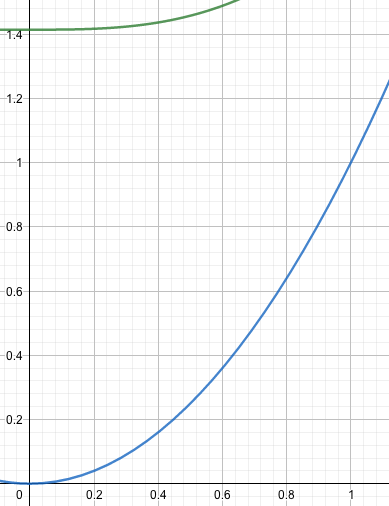
\includegraphics[scale=0.3]{region.png}
	\centering
	\caption{Gráfica de la región de integración.}
	\centering
\end{figure}

Notemos que la región comprendida se encuentra debajo de la función $x = \sqrt{y}$,
estando el intervalo en el eje $x$ limitado a la izquierda por la función
$x = \sqrt{y} $ y a la derecha por la constante $1$, de la misma forma, el
intervalo en el eje $y$ está limitado inferiormente por la constante $0$
y superiormente por la constante $1$.\\

Ahora, para modificar los límites de integración, observamos gráficamente que
los valores de $y$ quedarían limitados inferiormente por la constante $y = 0$
y superiormente por la función $x = \sqrt{y}$, equivalente a $y = x^2$.\\

Análogamente, para los valores de $x$, se encontarían limitados por la izquierda
por la constante $x = 0$ y por la derecha por $x = 1$. \\

Así, reescribimos los límites como:

	$$ \int_{0}^{1}\int_{0}^{x^2} \sqrt{(2 + x^3)} dy dx  $$

ahora, evaluando la integral, se tiene:
	$$   \int_{0}^{1}\int_{0}^{x^2} \sqrt{(2 + x^3)} dy dx  $$
	$$ = \int_{0}^{1}\sqrt{(2 + x^3)} \int_{0}^{x^2} dy dx  $$
	$$ = \int_{0}^{1}\sqrt{(2 + x^3)} y \Big|_{0}^{x^2} dx  $$
	$$ = \int_{0}^{1}\sqrt{(2 + x^3)} x^2  dx  $$

tomando $u = 2 + x^3$ se tiene:

	$$   \int_{0}^{1}\sqrt{(2 + x^3)} x^2  dx  $$
	$$ = \frac{1}{3} \int_{u(0)}^{u(1)}\sqrt{u} du  $$
	$$ = \frac{1}{3} \Eval{\frac{u^{\frac{3}{2}}}{\frac{3}{2}}}
						 {u(0)}{u(1)}  $$
	$$ = \frac{1}{3} \cdot \frac{2}{3} \Eval{u^{\frac{3}{2}}}
								 {u(0)}{u(1)}  $$

	$$ = \frac{2}{9} \Eval{ {2 + x^3}^{\frac{3}{2}} }{0}{1}  $$
	$$ = \frac{2}{9} \Bp {{3}^{\frac{3}{2}} -
						  {2}^{\frac{3}{2}}}  $$
	$$ = \frac{2}{9} \Bp {3 \sqrt{3} - 2 \sqrt{2} }  $$

\textbf{37.} \\

\[ \int \limits_0^1 \, \int \limits_{e^y}^e \frac{x}{\ln{x}} \, \text dx \, \text dy \]

Primero obtengamos los límites de integración reescribiendo la integral de $dx\,dy$ a $dy\,dx$ \\

Para los límites en $y$ tenemos $0$ para el inferior y $\ln{x}$ en donde $x = e^y$ por lo tanto $\ln{e^y} = \ln{x} $ entonces $y = \ln{x}$ para el superior. \\
Por otro lado para los límites en $x$ tenemos $1$ como el inferior y $e$ para el superior. \\ \\

Rescribiendo la integral tenemos:
$$\int_{1}^{e} \int_{0}^{\ln{x}} \frac{x}{\ln{x}} \, \text dy \, \text dx$$

Procediendo con la integral interior
$$ = \int_{1}^{e} \left[ \frac{x}{\ln{x}} \right]_{0}^{\ln{x}} \, \text dx$$

Evaluando
$$ = \int_{1}^{e} \frac{x}{\ln{x}} \left(\ln{x} - 0\right) \, \text dx$$

Llegamos a que
$$ = \int_{1}^{e} x \, \text dx$$

Evaluando
$$ = \frac{1}{2} \left[x^2\right]_{1}^{e}$$

Por lo tanto el resultado es
$$ = \frac{1}{2} \left(e^2 - 1\right)$$

\newpage

\textbf{60.} Show that for a right triangle the average distance from any point
in the triangle to one of the legs is one-third the length of the other leg.
(The legs of a right triangle are the two sides that are not the hypotenuse.) \\

\textbf{62.} Find the area of the crescent-moon shape with circular arcs as edges
and the dimensions shown in Figure 16.22. \\

Cómo la luna está compuesta de dos secciones circulares, sabemos que cada curva que contiene
a la región está conformada por un círculo de radio fijo.\\
Sean $E$ el círculo exterior e $I$ el círculo interior de la media luna.\\
Sea $r_E$ el radio del círculo exterior. Sabemos que este radio es de tamaño $r_E=4$ porque es cuándo
sabemos que la distancia entre el punto más alto, el más bajo y el extremo del lado dado son
consistentes. \\
Sea $r_I$ el radio del círculo interior $I$. Si "trazamos" una línea del punto más alto de la luna
al centro del círculo interior podemos formar un triángulo de altura $r_E=4$, hipotenusa de
tamaño $r_I$ y longitud horizontal de tamaño $r_I-2$ (Obtenemos esta medida trazando una línea del
centro de $I$ al centro del círculo $E$ que está a distancia $2$ del borde de $I$).\\
De esta manera, por el teorema de Pitágoras, tenemos que
\begin{equation}
	\begin{split}
		r_I^2	    &=4^2+(r_I)^2\\
			 	    &=16+r_I^2-4r_I+4\\
			 	    &=20+r_I^2-4r_I\\
		r_I^2-r_I^2 &=20-4r_I\\
		0 			&=20-4r_I\\
		4r_I		&=20\\
		r_I			&=5
	\end{split}
\end{equation}
Luego, si suponemos que el centro de $I$ está en el origen, tenemos porque
$$I={(x,y)|x^2+y^2=25}$$
y que
$$E={(x,y)|(x-(r_I-2))^2+ y^2=(x-3)^2+y^2=16}$$
De esta manera tenemo que el área de la luna se encuentra entre las curvas
$$x^2=25-y^2 \Rightarrow x=\sqrt{25-y^2}$$
y
$$(x-3)^2=16-y^2\Rightarrow x-3=\sqrt{16-y^2}\Rightarrow x=3+\sqrt{16-y^2}$$
Así, tenemos que el área de la media luna es:
\begin{equation}
	\begin{split}
		A&=\int_{-4}^4\int_{\sqrt{25-y^2}}^{3+\sqrt{16-y^2}}dxdy\\
		 &=\int_{-4}^4x\Big|_{\sqrt{25-y^2}}^{3+\sqrt{16-y^2}}dy\\
		 &=\int_{-4}^4\bp{3+\sqrt{16-y^2}-\sqrt{25-y^2}}dy\\
		 &=12+8\pi-25sin^{-1}(\tfrac{4}{5})\\
		 &=13.9504 \\
	\end{split}
\end{equation}
La penúltima ecuación se obtuvo de evaluar la antepenúltima ecuación en el software
de Mathematica y la última ecuación de evaluar este último resultado en la graficadora Desmos.

\textbf{Sección 16.3} \\

In Problems 14–18, decide whether the integrals are positive,negative, or zero.
Let $S$ be the solid sphere $x^2 + y^2 + z^2 \leq 1$, and $T$ be the top half of
be the right half of the sphere (with $x \geq 0$), and $L$ be the left half
this sphere (with $z \geq 0$), and $B$ be the bottom half (with $z \leq 0$), and $R$
(with $x \leq 0$). \\
\begin{itemize}
	\item[\textbf{14.}]$ \int _T e^z \, \text dV$\\
	Como $e^z$ es positiva en $T$, entonces la integral es positiva.

	\item[\textbf{15.}]$ \int _B e^z \, \text dV $\\
	Como $e^z$ es positiva en B, la integral es posiitva

	\item[\textbf{16.}]$\int _S \sin{z} \, \text dV$\\
	Tenemos que $\sin z$ es positiva en T y  es negativa con el mismo valor absoluto en la
	mitad inferior de $R$ por lo que la integral de $\sin z$ es cero.

	\item[\textbf{17.}]$ \int _T \sin{z} \, \text dV$\\
	Tenemos que el $sin z $ es positiva en $T$ por lo que la integral es positiva

	\item[\textbf{18.}]$\int _R \sin{z} \, \text dV $\\
	El $\sin z$ es positivo en la mitad superior de $R$ y negativa con el mismo valor absoluto
	en la mitad inferior de R por lo que la integral de $sin z$ es cero.
\end{itemize}

\textbf{31.} A trough with triangular cross-section lies along the $x$-axis for
$0 \leq x \leq 10$. The slanted sides are given by $z = y$ and $z = -y$ for
$0 \leq z \leq 1$ and the ends by $x = 0$ and $x = 10$, where $x, y, z$ are in meters.
The trough contains a sludge whose density at the point $(x, y, z)$ is
$\delta = e^{-3x}$ kg per $m^3$. \\

\textbf{a)} Express the total mass of sludge in the trough in terms of triple
integrals. \\

\textbf{b)} Express the total mass of sludge in the trough in terms of triple
integrals. \\

\textbf{55.} $E$ is the region bounded by $x = 0, y = 0, z = 0, z = 2,$
and $2x + 4y + z = 4$. \\

\textbf{57.} Figure 16.28 shows part of a spherical ball of radius 5 cm.
Write an iterated triple integral which represents the volume of this region. \\

\begin{figure}[h]
%\includegraphics[scale=0.5]{images/img4.png}
\centering
\end{figure}

Si consideramos que ese corte de la esfera se encuentra centrado en el origen,
entonces podemos notar que si su radio es de 5cm y tiene una altura de 2cm,
entonces definimos el sólido con las desigualdades:

\[ 0 \leq z \leq 2, -5 \leq x \leq 5, - \sqrt{25 - x^2} \leq y \leq \sqrt{25 - x^2}\]

Entonces:

\[ \iiint \limits_G z(x,y) dV = \int \limits_0^2 \int \limits_{-5}^5
        \int \limits_{- \sqrt{25 - x^2}}^{\sqrt{25 - x^2}} z(x,y) \, \text dy \, \text dx \, \text dz  \]


\textbf{66.} Find the center of mass of the tetrahedron that is bounded by the
$xy, yz, xz$ planes and the plane $x + 2y + 3z = 1$. Assume the density is
1 $gm/cm^3$ and $x, y, z$ are in centimeters. \\
Sabemos que $m = \int_W 1dV$. Estableciendo los límites en función de $z$ y desta en
términos de $y$
tenemos que
$$z=\frac{1-x-\tfrac{y}{2}}{3}$$ y
$$y=\frac{1-x}{2}$$
Entonces,
\begin{equation}
	\begin{split}
		\int_WdV&=\int_0^1\tsint{\frac{1-x}{2}}\tsint{\frac{1-x-2y}{3}}dzdydx\\
			    &=\int_0^1\tsint{\frac{1-x}{2}}z\bigg|_0^{\frac{1-x-2y}{3}}dydx\\
				&=\int_0^1\tsint{\frac{1-x}{2}}\frac{1-x-2y}{3}dydx\\
				&=\frac{1}{3}\int_0^1\tsint{\frac{1-x}{2}}\bp{1-x-2y}\ dydx\\
				&=\frac{1}{3}\int_0^1y-xy-y^2\bigg|_0^{\frac{1-x}{2}}dx\\
				&=\frac{1}{3}\int_0^1\Bp{\bp{\tfrac{1}{2}-\tfrac{x}{2}}-\bp{\tfrac{x}{2}
					-\tfrac{x^2}{2}}-\tfrac{1}{2}\bp{\tfrac{1}{2}-x+\tfrac{x^2}{2}}}dx\\
				&=\frac{1}{6}\int_0^1\Bp{\bp{1-x}-\bp{x-x^2}-\tfrac{1}{2}\bp{1-x+x^2}}dx\\
				&=\frac{1}{6}\int_0^1\Bp{\bp{1-2x-x^2}-\tfrac{1}{2}\bp{1-x+x^2}}dx\\
				&=\frac{1}{6}\int_0^1\Bp{\bp{1-2x-x^2}-\bp{\tfrac{1}{2}-\tfrac{x}{2}+\tfrac{x^2}{2}}}dx\\
				&=\tfrac{1}{6}\Bp{\bp{x-x^2-\tfrac{x^3}{3}-\tfrac{x}{2}+\tfrac{x^2}{4}
					-\tfrac{x^3}{6}}\Big|_0^1}\\
				&=\tfrac{1}{6}\Bp{1-1-\tfrac{1}{3}-\tfrac{1}{2}+\tfrac{1}{4}-\tfrac{1}{6}}\\
				&=\tfrac{1}{6}\Bp{\tfrac{12-12+4-6+3-2}{12}}\\
				&=\tfrac{1}{6}\Bp{-\tfrac{1}{12}}\\
				&=-\tfrac{1}{36}\\
	\end{split}
\end{equation}
Pero cómo la masa siempre es positiva, entonces
\[\int_WdV=\Big|-\tfrac{1}{36}\Big|=\tfrac{1}{36}\]
Entonces, $\frac{1}{m}=\frac{1}{\frac{1}{36}}=36$
De esto, tenemos las siguientes tres ecuaciones con sus resultados correspondientes
evaluados en un CAS:
\begin{equation}
	\begin{split}
		\bar{x}&=36\int_WdV\\
			   &=36\int_0^1\tsint{\frac{1-x}{2}}\tsint{\frac{1-x-2y}{3}}xdzdydx\\
			   &=36\frac{1}{144}\\
			   &=\frac{1}{4}\\
		\bar{y}&=36\int_WdV\\
			   &=36\int_0^{\tfrac{1}{2}}\tsint{1-2y}\tsint{\frac{1-x-2y}{3}}ydzdydx\\
			   &=36\frac{1}{288}\\
			   &=\frac{1}{8}\\
		\bar{z}&=36\int_WdV\\
			   &=36\int_0^{\tfrac{1}{3}}\tsint{1-3z}\tsint{\frac{1-x-3z}{2}}zdzdydx\\
			   &=36\frac{1}{432}\\
			   &=\frac{1}{12}\\
	\end{split}
\end{equation}


Problems 67–69 concern a rotating solid body and its \textit{moment of inertia}
about an axis; this moment relates angular acceleration to torque (an analogue
of force). For a body of constant density and mass $m$ occupying a region $W$
of volume $V$ , the moments of inertia about the coordinate axes are

\[I_x = \tfrac{m}{V} \int _W (y^2 + z^2) \, \text d V \]

\[I_y = \tfrac{m}{V} \int _W (x^2 + z^2) \, \text d V \]

\[I_z = \tfrac{m}{V} \int _W (x^2 + z^2) \, \text d V \]

\textbf{67.} Find the moment of inertia about the $z$-axis of the rectangular
solid of mass $m$ given by $0 \leq x \leq 1, 0 \leq y \leq 2, 0 \leq z \leq 3$. \\

Como nos  pide encontrar el momento de inercia respecto al eje $z$ entonces tomamos de las ecuaciones de arriba y tomamos $I_z$
\[I_{z} = \frac{m}{V} \int_W (x^2+y^2) dV\]
Por lo que tenemos que integrar : $\frac{m}{6} \int_W x^2+ y^2 dV$\\
Sustituyendo las regiones de integración:
\[\frac{m}{6} \int_0^1 \int_0^2 \int_0^3 x^2 + y^2 dz dy dx\]
Resolveremos en el siguiente orden:
\[\frac{m}{6} \left[ \int_0^1\left[ \int_0^2\left[ \int_0^3 x^2 + y^2 dz \right] dy \right] dx \right] \]
Como en $\int_0 ^3 x^2+ y^2 dz$ es una integral respecto a $z$ y no existe esta variable dentro
de la ecuación $x^2+ y^2$ entonces evaluamos en $z = 3$ y :
\[\frac{m}{6} \int_0^1 \int_0^2 3\left( x^2+y^2 \right) dy dx\]
Ahora integramos respecto a $y$:
\[\frac{m}{2} \int_0^1 \left( x^2y+ y^3/3 \right) \vert_0^2 dx\]
Evaluamos con $y= 2$ y con $y= 0$ y tenemos que :
\[\frac{m}{2} \int_0^1 \left( 2x^2+ 8/3 \right) dx = \frac{5m}{3}\]
Calculamos la integral respecto a $x$
\[\frac{m}{2} \left( 2x^3/3 + 8/3 x \right) \vert_0^1\]
Are the statements in Problems 74–83 true or false? Give reasons for your answer. \\

\textbf{75.} The region of integration of the triple iterated integral
$\int_0^1 \int_0^1 \int_0^x f dz dy dx $ lies above a square in the $xy$-plane
and below a plane. \\

\textbf{78.} The iterated integrals $\int_{-1}^1 \int_0^1 \int_0^{1-x^2} f dz dy dx $
and $\int_0^1 \int_0^1 \int_{-\sqrt{1-z}}^{\sqrt{1-z}} f dz dy dx $ are equal. \\

\textbf{80.} If $W$ is the unit cube $0 \leq x \leq 1, 0 \leq y \leq 1, 0 \leq z \leq 1$
and $ \int _W f \, \text dV = 0$, then $f = 0$ everywhere in the unit. \\

Falso, si la función $f$ es simétrica con respecto a el plano $xy$, provoca que al
realizar la integral en la región, el volumen inferior al plano se cancele con el
volumen superior. Por ejemplo, si $f(x,y,z) = \frac{1}{2} - x$, el resultado
de la integral es:

\begin{equation}
\begin{split}
        \int_0^1 \int_0^1 \int_0^1 \left( \frac{1}{2} - x \right) \, \text dx \, \text dy \, \text dz
        &= \int_0^1 \int_0^1 \left( \frac{1}{2}x - \frac{x^2}{2} \right) \Bigg|_0^1 \, \text dy \, \text dz \\ \notag
        &= \int_0^1 \int_0^1 \left( \frac{1}{2} - \frac{1}{2} \right) \, \text dy \, \text dz \\ \notag
        &= \int_0^1 \int_0^1 0 \, \text dy \, \text dz = 0 \\ \notag
\end{split}
\end{equation}

\end{document}
